\ngeq\section{Brikker}

Formålet med at implementere brikker i spillet var at give gameplayet en helt ny dimension. 

\begin{itemize}
\item \textbf{Tegne Brikker.} Du kan se et billede af brikkerne her \ref{fig:brik}
For lettest at kunne holde styr på brikkerne har vi lavet en struct, \texttt{Brick} der repræsenterer en brik. Den indeholder position i x- og y-koordinater, bredde, højde og brikkens liv. Brikkerne i en bane er gemt i et array: \texttt{Brick bricks[BRICK\_TABLE\_HEIGHT][BRICK\_TABLE\_WIDTH];}. Når banen initialiseres gennemløbes dette array og hver brik tildeles koordinater, bredde, højde og liv. Efter dette tegnes brikken. Hvis brikken har 0 liv svarer det til at der ikke er en brik. Ved at give de forskellige brikker i array'et forskellige antal liv kan man lave forskellige brikmønstre og på den måde kan man lave forskellige baner. 
%\begin{itemize}
\item \textbf{Baner gemt i et array i ROM'en.} Vi har valgt at hardcode brikkernes bredde og højde for at spare plads når vi gemmer banerne i ROM'en. På denne måde kan en bane i ROM'en gemmes i arrayet \texttt{unsigned char rom levels[4][BRICK\_TABLE\_HEIGHT][BRICK\_TABLE\_WIDTH]}. Dette arrray er et tredimensionalt array af chars. Det indeholder fire "lag" der hver indeholder de todimensionale data til en bane. Værdien af hver char er antallet af liv den tilsvarende brik får. 
\begin{lstlisting}
{
		{ 0, 0, 0, 0, 0, 0, 0, 0, 0, 0, 0, 0, 0, 0 },
		{ 0, 0, 0, 0, 0, 0, 0, 0, 0, 0, 0, 0, 0, 0 },
		{ 0, 0, 0, 0, 0, 0, 0, 0, 0, 0, 0, 0, 0, 0 },
		{ 0, 0, 0, 0, 0, 0, 0, 0, 0, 0, 0, 0, 0, 0 },
		{ 0, 0, 0, 0, 0, 0, 0, 0, 0, 0, 0, 0, 0, 0 },
		{ 0, 0, 0, 0, 0, 0, 0, 0, 0, 0, 0, 0, 0, 0 },
		{ 0, 1, 1, 1, 1, 1, 1, 1, 1, 1, 1, 1, 1, 0 },
		{ 0, 1, 1, 1, 1, 1, 1, 1, 1, 1, 1, 1, 1, 0 },
		{ 0, 2, 2, 2, 2, 2, 2, 2, 2, 2, 2, 2, 2, 0 },
		{ 0, 3, 3, 3, 3, 3, 3, 3, 3, 3, 3, 3, 3, 0 },
		{ 0, 4, 4, 4, 4, 4, 4, 4, 4, 4, 4, 4, 4, 0 },
		{ 0, 0, 0, 0, 0, 0, 0, 0, 0, 0, 0, 0, 0, 0 },
		{ 0, 0, 0, 0, 0, 0, 0, 0, 0, 0, 0, 0, 0, 0 },
		{ 0, 0, 0, 0, 0, 0, 0, 0, 0, 0, 0, 0, 0, 0 },
		{ 0, 0, 0, 0, 0, 0, 0, 0, 0, 0, 0, 0, 0, 0 },
		{ 0, 0, 0, 0, 0, 0, 0, 0, 0, 0, 0, 0, 0, 0 },
		{ 0, 0, 0, 0, 0, 0, 0, 0, 0, 0, 0, 0, 0, 0 },
		{ 0, 0, 0, 0, 0, 0, 0, 0, 0, 0, 0, 0, 0, 0 },
		{ 0, 0, 0, 0, 0, 0, 0, 0, 0, 0, 0, 0, 0, 0 },
	},
\end{lstlisting}



%\end{itemize}
\item Tjekke om man rammer brikker
\begin{itemize}
\item Højre/venstre og oppe/nede
\item Kanter?
\end{itemize}
\item Trække liv fra brikkerne
\item Lave deflect på baggrund af om der er brikker omkring brikken
\begin{itemize}
\item Forklare tilfældene med at ramme to brikker af gangen
\item Forklare tilfældene med at ramme flere hjørner
\end{itemize}
\item Briklogik korrigeret fordi der bevæges 2 karakterer i x-retningen
\end{itemize}


\begin{figure}[h!]
\centering
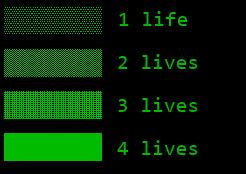
\includegraphics[scale=0.5]{figs/brikker.png}
\caption{Sådan ser brikkerne ud.}
\label{fig:brik}
\end{figure}